\chapter{Taxa Assemblage in Reference Sites}


\begin{figure}[htbp]
    \centering
    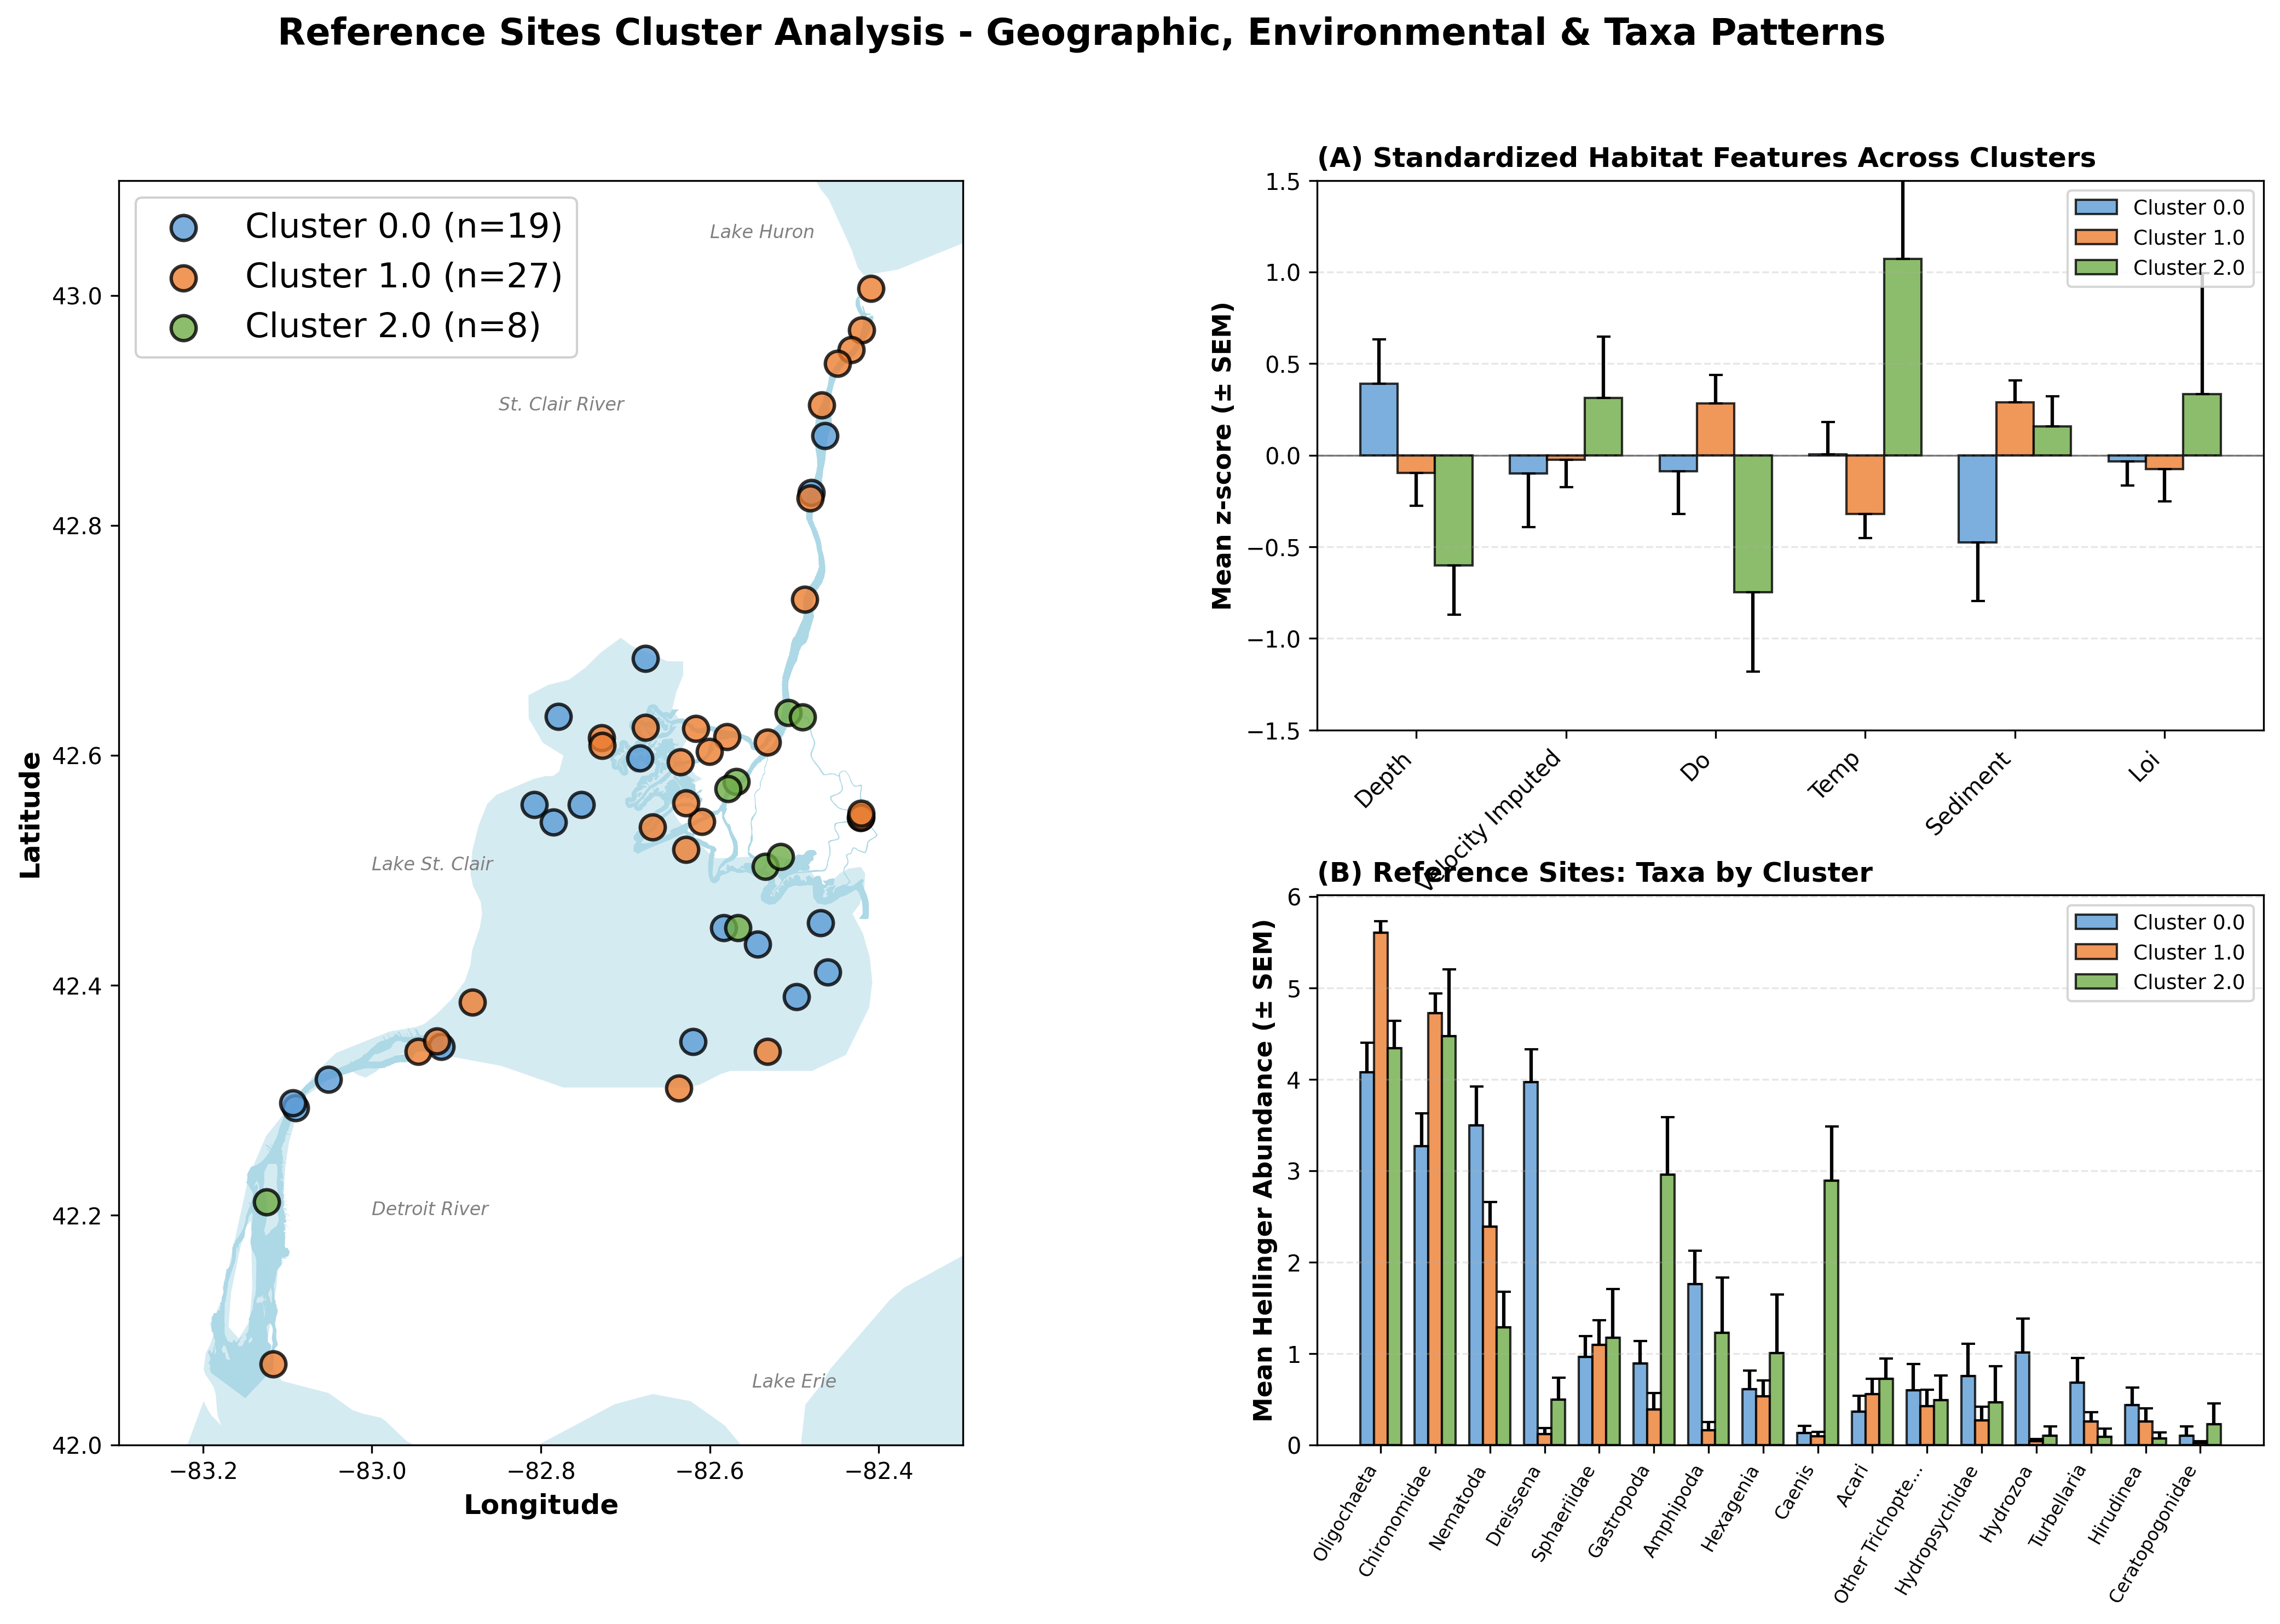
\includegraphics[width=0.9\textwidth]{../results/figures/02_taxa_assemblage_in_refs/figure2_cluster_visualization.png}
    \caption{Cluster Visualization}
    \label{fig:02_cluster_visualization}
\end{figure}

\begin{figure}[htbp]
    \centering
    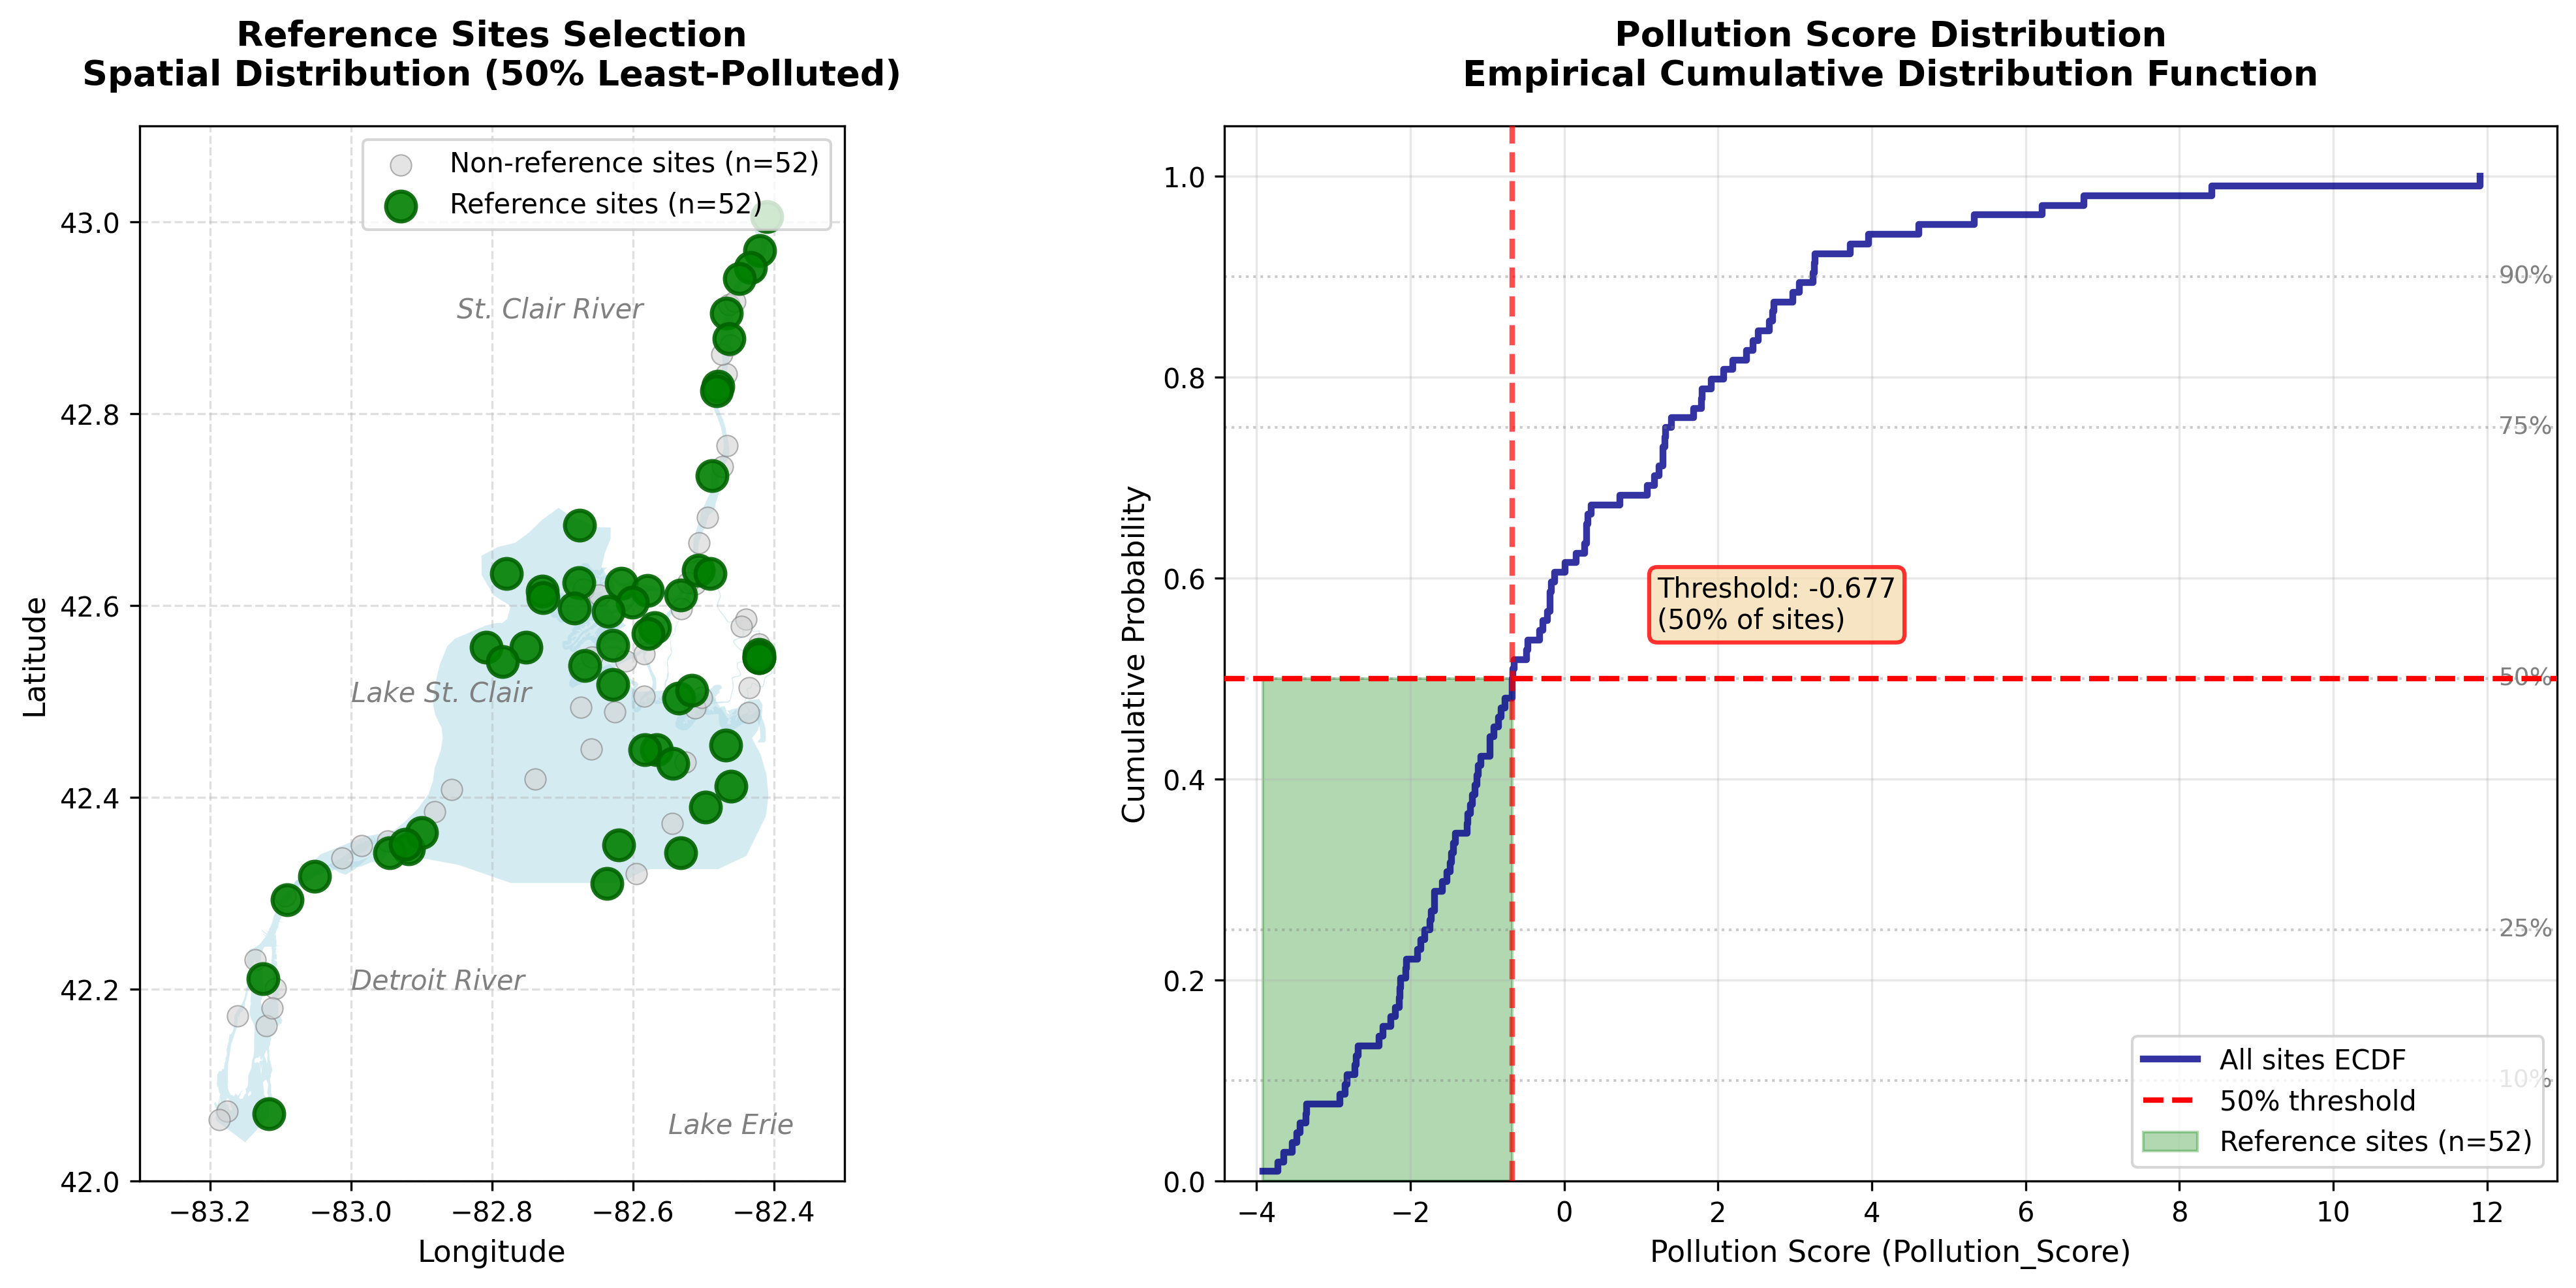
\includegraphics[width=0.9\textwidth]{../results/figures/02_taxa_assemblage_in_refs/figure2_reference_selection.png}
    \caption{Reference Selection}
    \label{fig:02_reference_selection}
\end{figure}

% \begin{figure}[htbp]
%     \centering
%     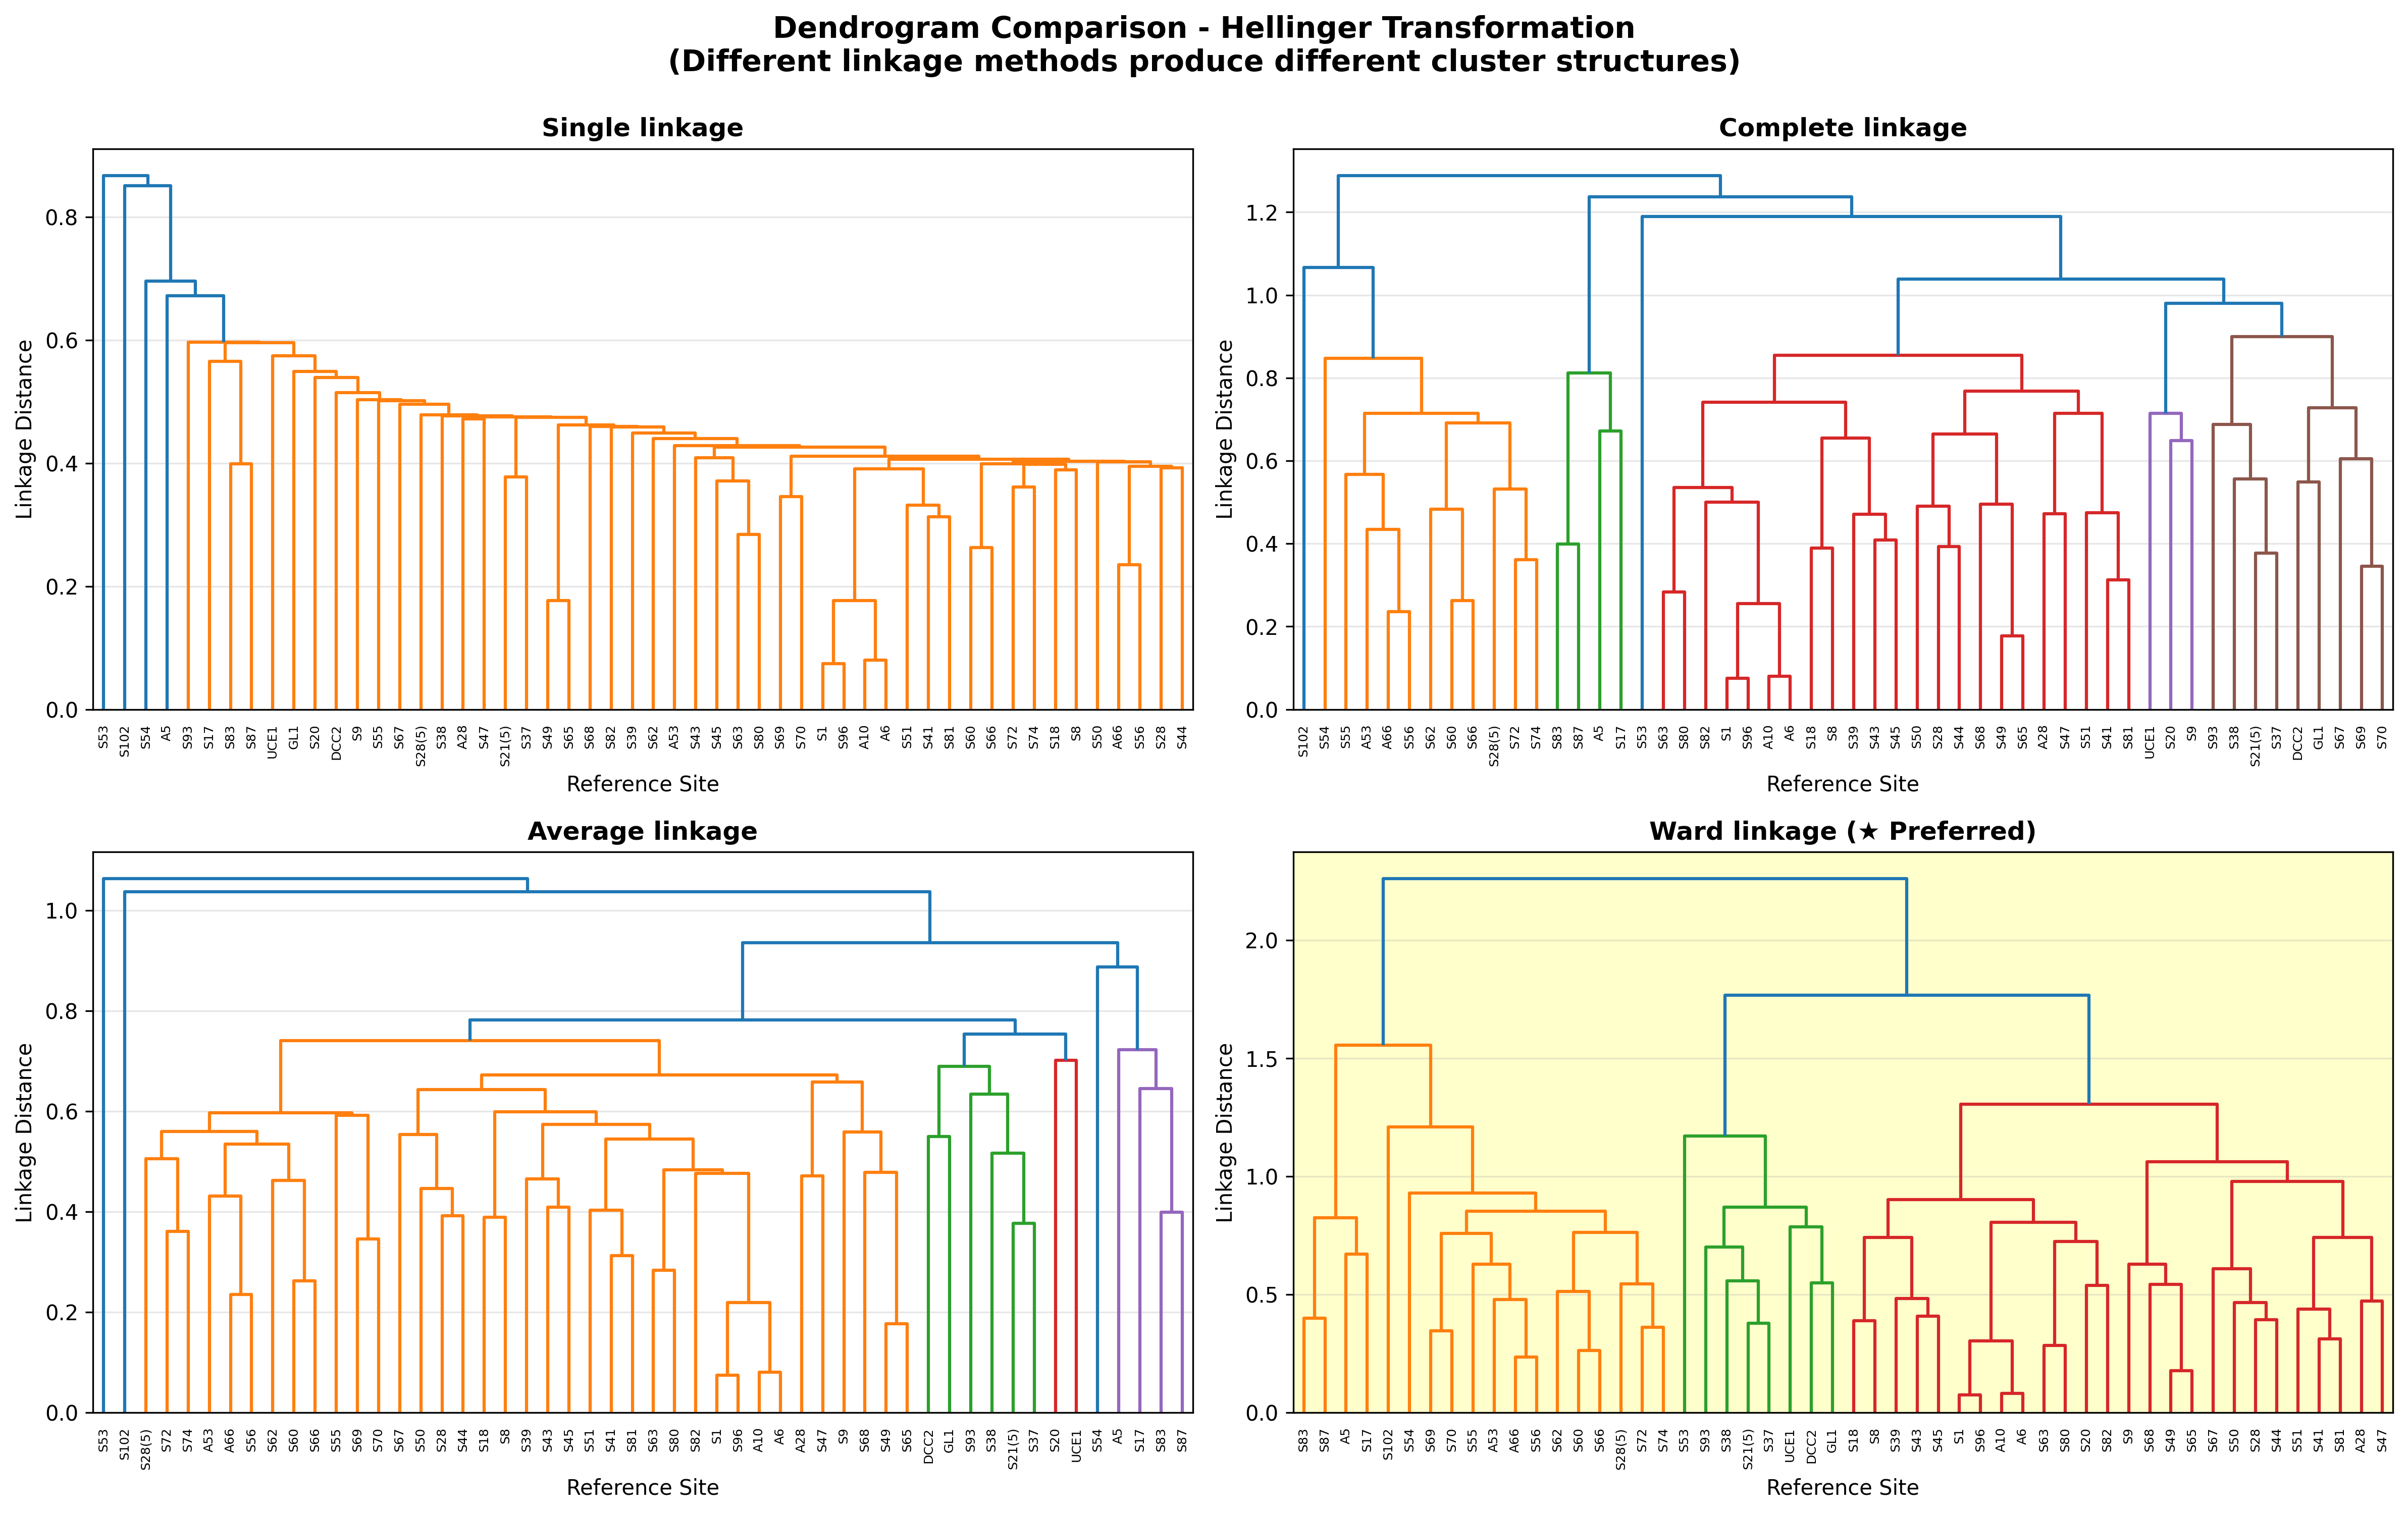
\includegraphics[width=0.9\textwidth]{../results/figures/02_taxa_assemblage_in_refs/figure3_dendrogram_comparison.png}
%     \caption{Dendrogram Comparison}
%     \label{fig:02_dendrogram_comparison}
% \end{figure}

% \begin{figure}[htbp]
%     \centering
%     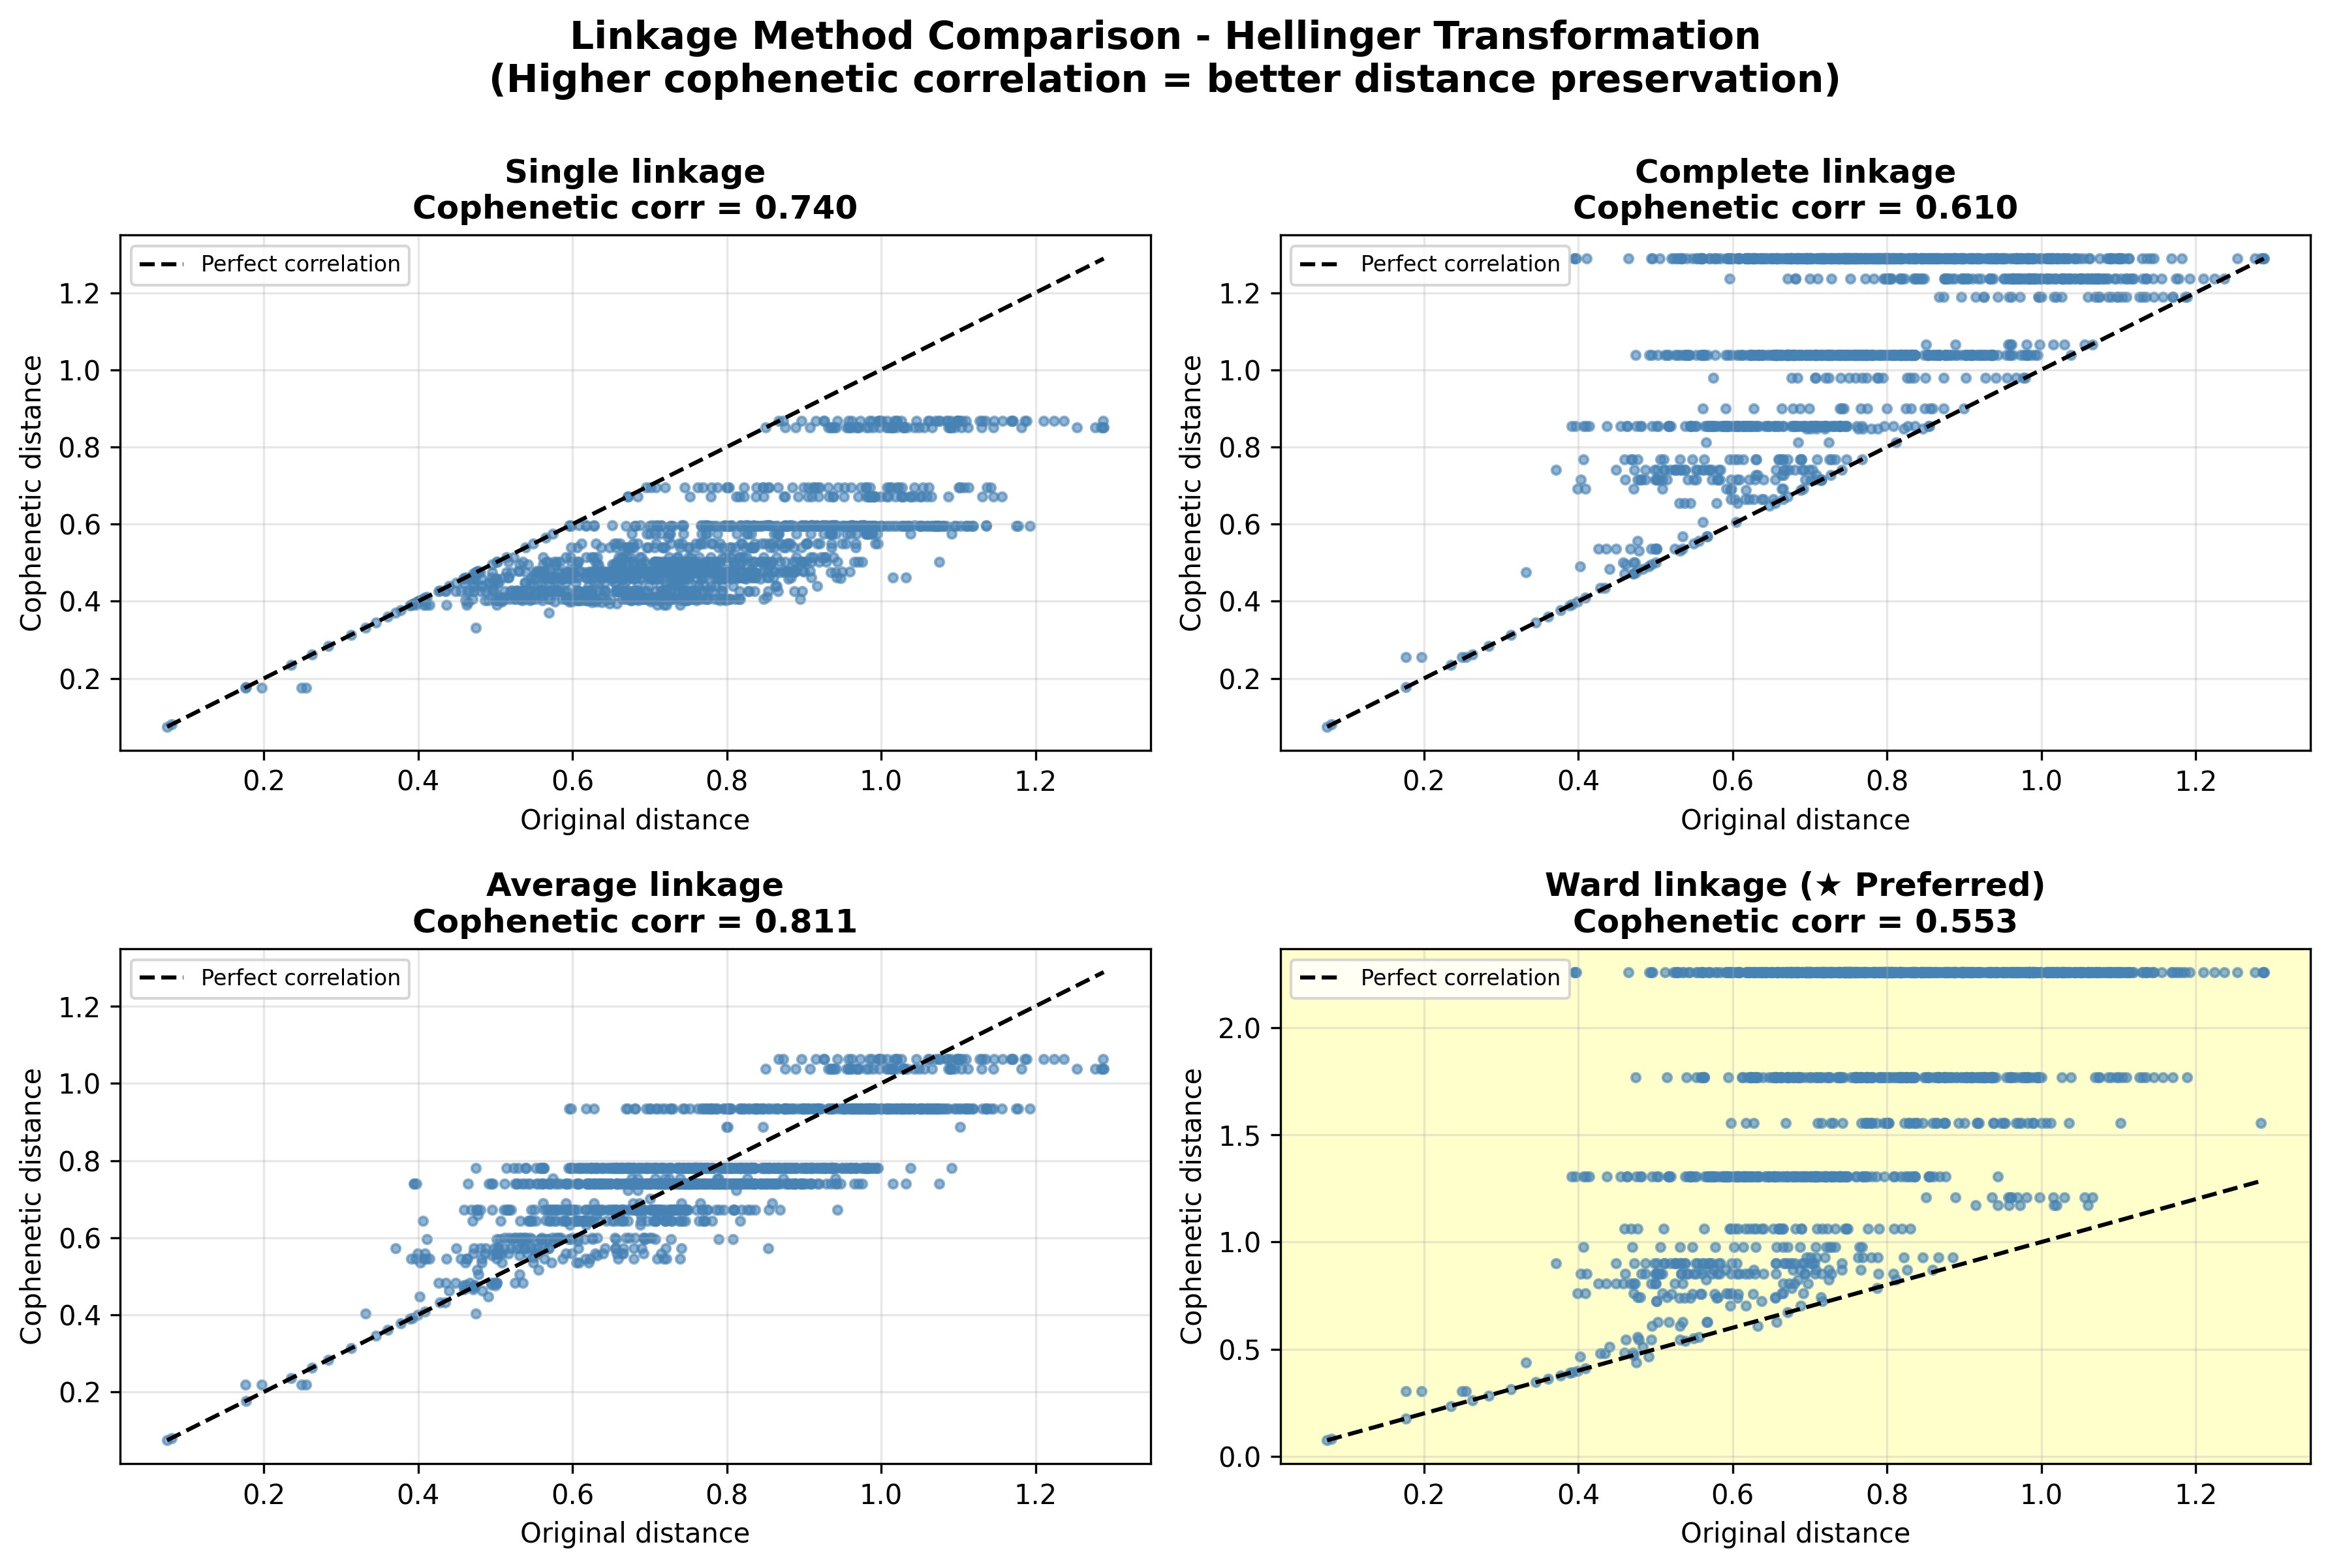
\includegraphics[width=0.9\textwidth]{../results/figures/02_taxa_assemblage_in_refs/figure4_linkage_comparison.png}
%     \caption{Linkage Comparison}
%     \label{fig:02_linkage_comparison}
% \end{figure}

\begin{figure}[htbp]
    \centering
    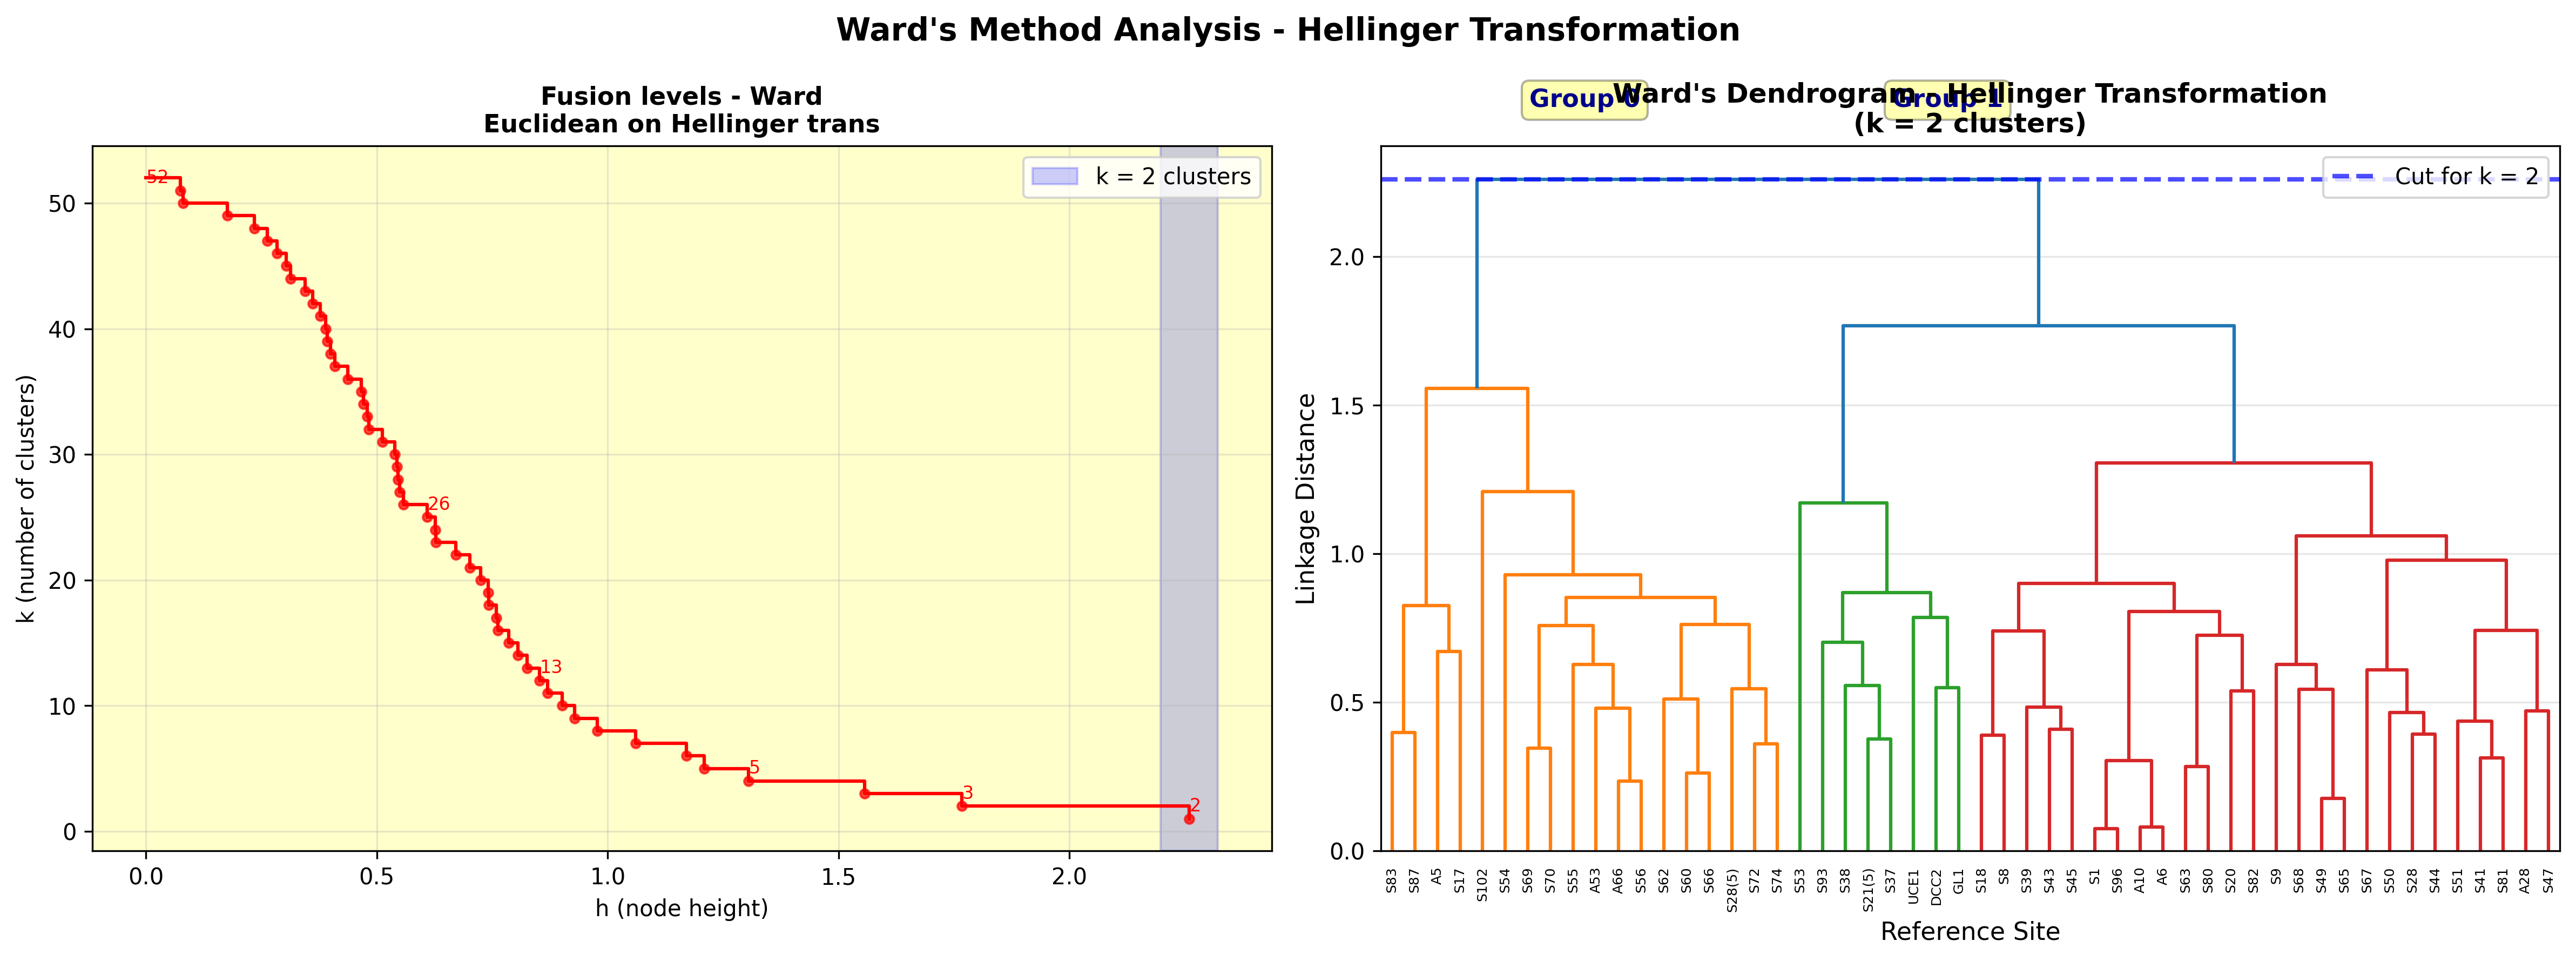
\includegraphics[width=0.9\textwidth]{../results/figures/02_taxa_assemblage_in_refs/figure5_ward_analysis.png}
    \caption{Ward Analysis}
    \label{fig:02_ward_analysis}
\end{figure}

\begin{figure}[htbp]
    \centering
    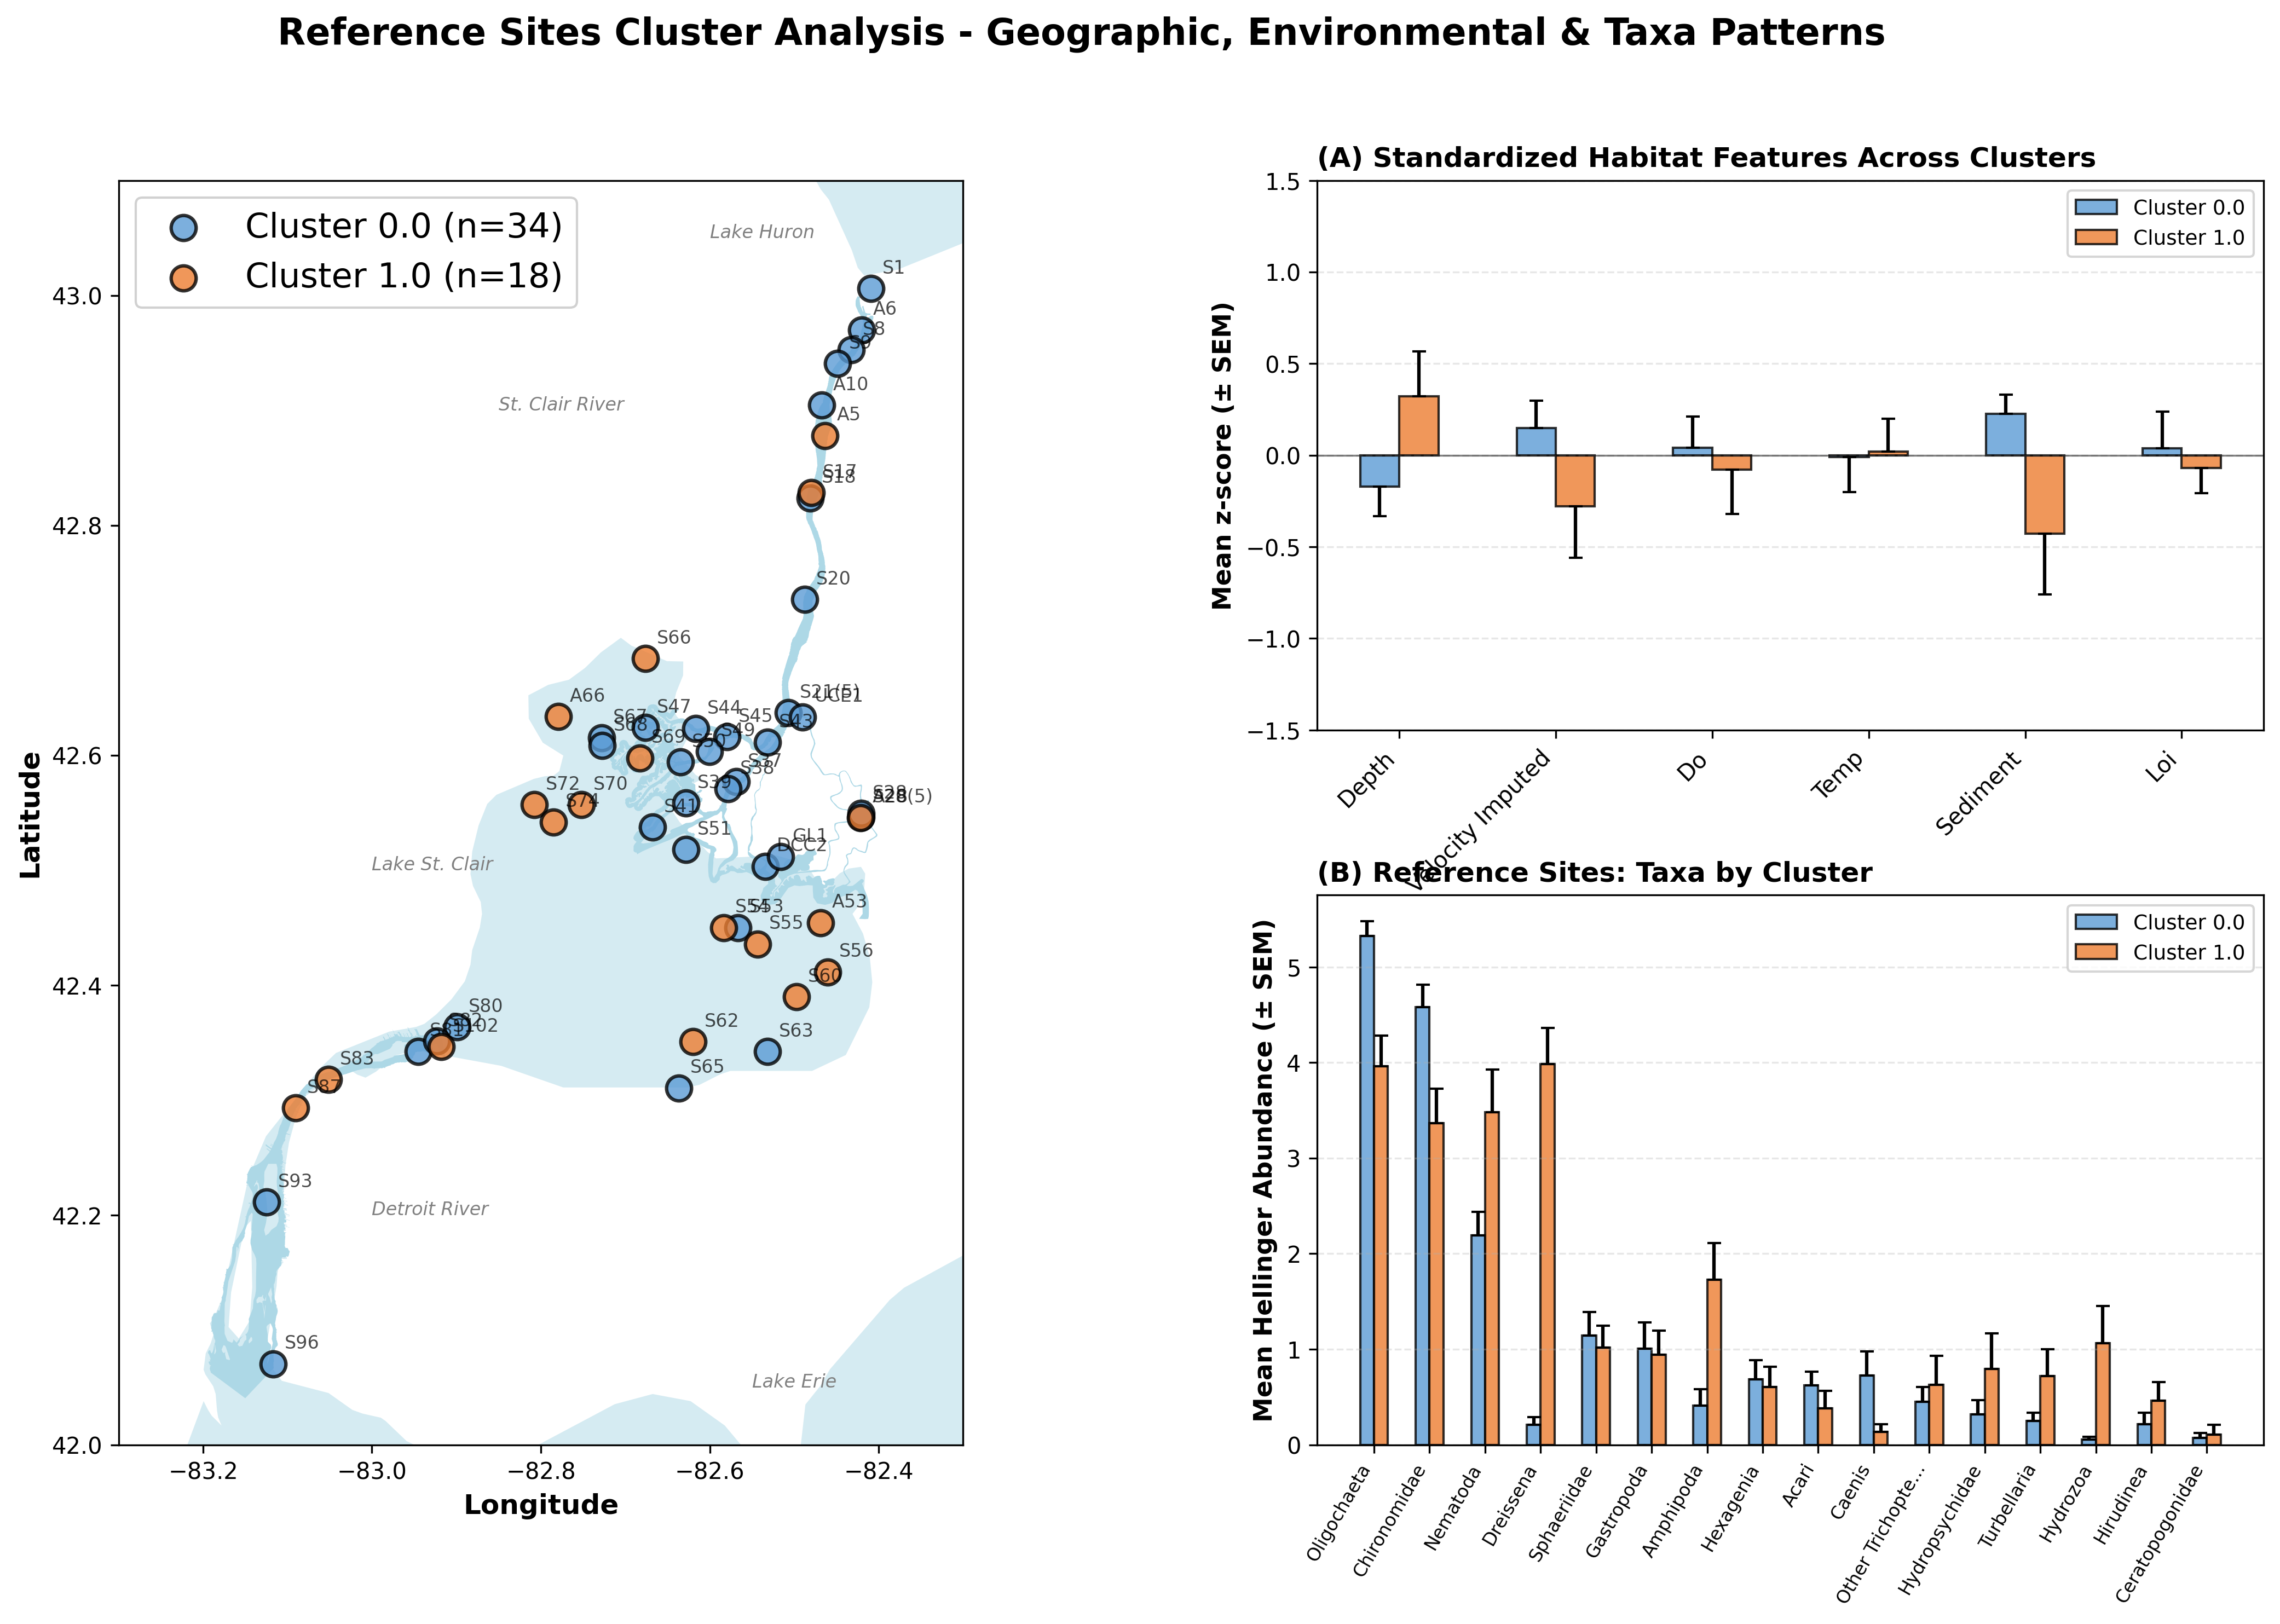
\includegraphics[width=0.9\textwidth]{../results/figures/02_taxa_assemblage_in_refs/figure6_cluster_visualization.png}
    \caption{Cluster Visualization Final}
    \label{fig:02_cluster_visualization_final}
\end{figure}



% =============================================================================
% Environmental Characteristics by Cluster
% =============================================================================
\begin{table}[htbp]
\centering
\footnotesize
\caption{Environmental Characteristics by Cluster (Reference Sites Only)}
\label{tab:02_env_characteristics}
\begin{tabular}{@{}lccc>{\centering\arraybackslash}p{1.5cm}@{}}
\toprule
Variable & Cluster 0 & Cluster 1 & Cluster 2 & F-stat \\
\midrule
Depth (m) & 4.48 $\pm$ 2.74 & 3.50 $\pm$ 2.48 & 2.06 $\pm$ 2.04 & 2.62 \\
Velocity (m/sec) & 0.09 $\pm$ 0.13 & 0.12 $\pm$ 0.09 & 0.16 $\pm$ 0.11 & 1.20 \\
DO Bottom (mg/L) & 9.44 $\pm$ 0.96 & 9.77 $\pm$ 0.73 & 8.83 $\pm$ 1.12 & 3.68* \\
Temperature (\textdegree C) & 20.64 $\pm$ 1.38 & 19.90 $\pm$ 1.27 & 22.47 $\pm$ 2.90 & 7.90** \\
MPS (Phi) & 0.85 $\pm$ 1.34 & 1.50 $\pm$ 0.60 & 1.38 $\pm$ 0.46 & 2.88. \\
LOI (\%) & 1.77 $\pm$ 0.68 & 1.75 $\pm$ 1.04 & 2.20 $\pm$ 2.14 & 0.49 \\
\midrule
Sample size (n) & 18 & 28 & 8 & \\
Environment Type & Fine Silt & Silt / Organic Rich & Coarse Gravel/Cobble & \\
\bottomrule
\end{tabular}
\begin{flushleft}
\footnotesize{Significance: *** p$<$0.001, ** p$<$0.01, * p$<$0.05, . p$<$0.1}
\end{flushleft}
\end{table}

% =============================================================================
% Top Taxa Abundance by Cluster
% =============================================================================
\begin{table}[htbp]
\centering
\small
\caption{Top Taxa Abundance by Cluster (Reference Sites Only)}
\label{tab:02_taxa_abundance}
\begin{tabular}{@{}lccc>{\centering\arraybackslash}p{1.6cm}@{}}
\toprule
Taxon & Cluster 0 & Cluster 1 & Cluster 2 & F-stat \\
\midrule
Oligochaeta & 3.964 & 5.614 & 4.337 & 17.52*** \\
Chironomidae & 3.365 & 4.689 & 4.471 & 4.90* \\
Nematoda & 3.478 & 2.468 & 1.283 & 5.71** \\
Dreissena & 3.982 & 0.114 & 0.495 & 86.56*** \\
Sphaeriidae & 1.014 & 1.057 & 1.169 & 0.04 \\
Gastropoda & 0.940 & 0.373 & 2.957 & 16.36*** \\
Amphipoda & 1.728 & 0.150 & 1.227 & 10.27*** \\
Hexagenia & 0.604 & 0.544 & 1.006 & 0.59 \\
Acari & 0.382 & 0.566 & 0.722 & 0.56 \\
Caenis & 0.134 & 0.088 & 2.892 & 57.94*** \\
\bottomrule
\end{tabular}
\begin{flushleft}
\footnotesize{Showing top 10 of 16 total taxa. Significance: *** p$<$0.001, ** p$<$0.01, * p$<$0.05, . p$<$0.1}
\end{flushleft}
\end{table}

% =============================================================================
% Significant Taxa Descriptions with Images
% =============================================================================
\newpage
\section{Significant Indicator Taxa}


Seven taxa showed statistically significant differences in abundance among the three reference site clusters (Table~\ref{tab:02_taxa_abundance}), indicating their potential as habitat indicators.

\begin{wrapfigure}{r}{0.3\textwidth}
    \centering
    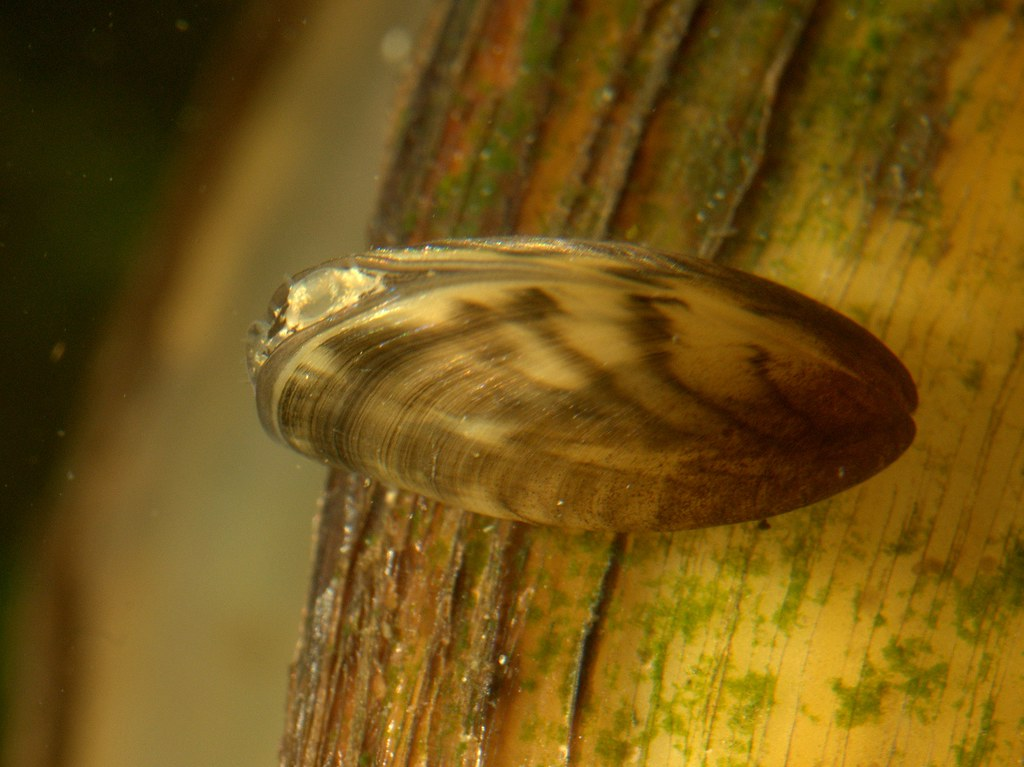
\includegraphics[width=0.28\textwidth]{../data/taxa_images/Dreissena_image.jpg}
    \caption{Dreissena}
    \label{fig:dreissena}
\end{wrapfigure}
\noindent\textbf{Dreissena} (F = 86.56***) exhibited the most significant difference among clusters, with extremely high abundance in Cluster 0 (3.982) but nearly absent in Clusters 1 (0.114) and 2 (0.495). Zebra and quagga mussels strongly characterize hard substrate environments with good water circulation. These invasive bivalves are filter feeders that can significantly alter local nutrient dynamics and water clarity. Their presence typically indicates stable, hard substrates such as rocks, cobbles, or artificial structures. \lipsum[1][1-4]

\begin{wrapfigure}{l}{0.3\textwidth}
    \centering
    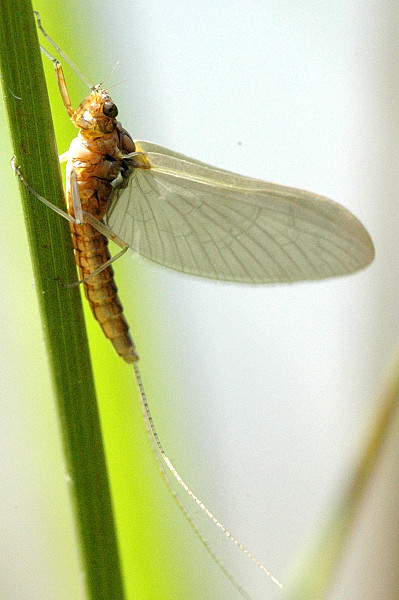
\includegraphics[width=0.28\textwidth]{../data/taxa_images/Caenis_image.jpg}
    \caption{Caenis}
    \label{fig:caenis}
\end{wrapfigure}
\noindent\textbf{Caenis} (F = 57.94***) was predominantly found in Cluster 2 (2.892) with minimal presence in Clusters 0 (0.134) and 1 (0.088). These small mayflies are characteristic of erosional, shallow-water environments with moderate current. They are collector-gatherers that feed on fine particulate organic matter and are moderately tolerant to pollution, making them useful indicators of intermediate water quality conditions in lotic systems. \lipsum[2][1-4]

\lipsum[2]

\begin{wrapfigure}{r}{0.3\textwidth}
    \centering
    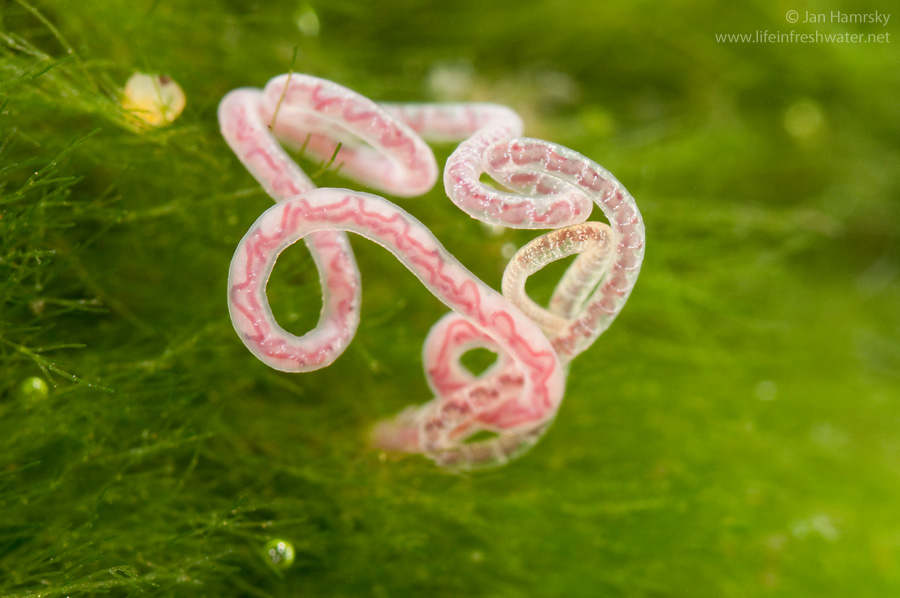
\includegraphics[width=0.28\textwidth]{../data/taxa_images/Oligochaeta_image.jpg}
    \caption{Oligochaeta}
    \label{fig:oligochaeta}
\end{wrapfigure}
noindent\textbf{Oligochaeta} (F = 17.52***) showed the highest abundance in Cluster 1 (5.614) compared to Cluster 0 (3.964) and Cluster 2 (4.337). These segmented worms are important indicators of organic enrichment in fine-grained sediments. They play a crucial role in sediment bioturbation and nutrient cycling, and their high abundance often indicates depositional environments with accumulated organic matter. \lipsum[3][1-4]


\begin{wrapfigure}{l}{0.3\textwidth}
    \centering
    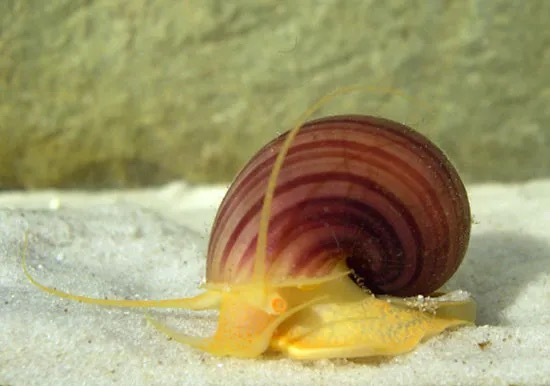
\includegraphics[width=0.28\textwidth]{../data/taxa_images/Gastropoda_image_converted.jpg}
    \caption{Gastropoda}
    \label{fig:gastropoda}
\end{wrapfigure}
\noindent\textbf{Gastropoda} (F = 16.36***) showed highest abundance in Cluster 2 (2.957), moderate in Cluster 0 (0.940), and lowest in Cluster 1 (0.373). Freshwater snails prefer hard substrates and well-oxygenated shallow waters where they graze on periphyton and detritus. Their distribution patterns often reflect substrate type, food availability, and calcium concentrations in the benthic environment. \lipsum[4][1-4]

\begin{wrapfigure}{r}{0.3\textwidth}
    \centering
    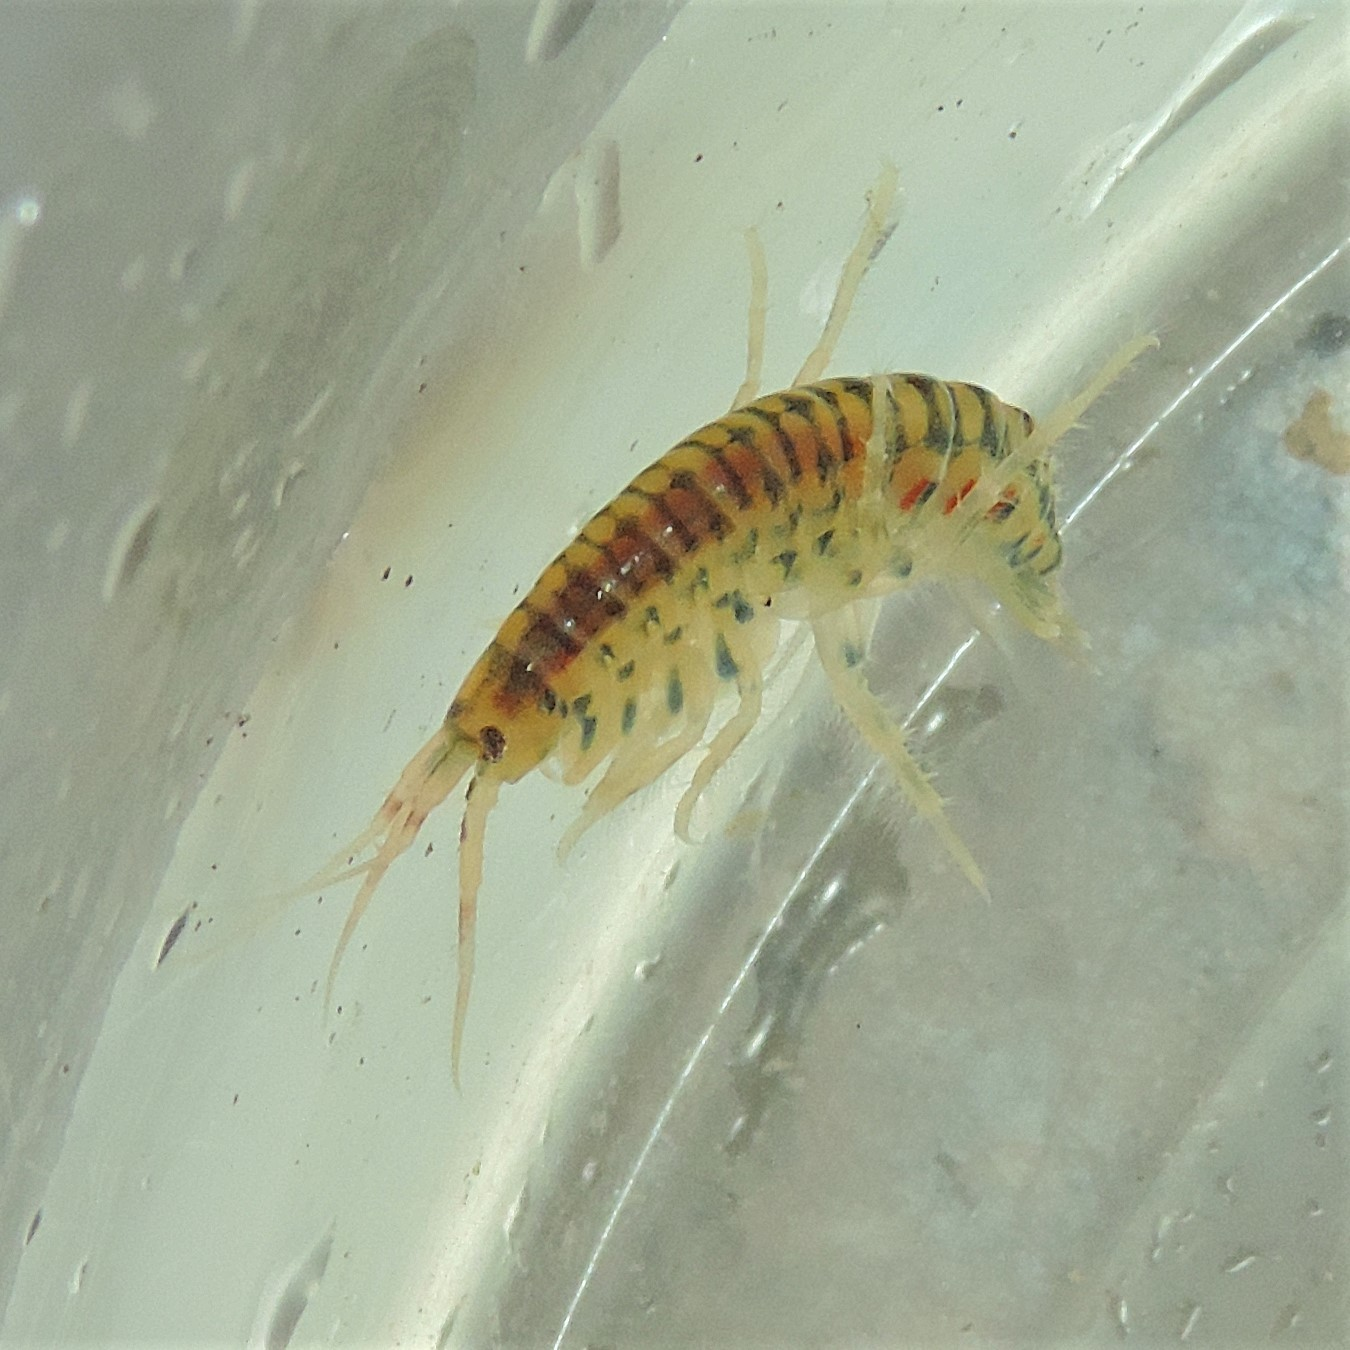
\includegraphics[width=0.28\textwidth]{../data/taxa_images/Amphipoda_image.jpg}
    \caption{Amphipoda}
    \label{fig:amphipoda}
\end{wrapfigure}
\noindent\textbf{Amphipoda} (F = 10.27***) was most abundant in Cluster 0 (1.728), moderate in Cluster 2 (1.227), and nearly absent in Cluster 1 (0.150). Scuds are sensitive indicators preferring clean, well-oxygenated habitats with structured substrates. They are important prey items for fish and serve as shredders and detritivores in the benthic food web, processing coarse particulate organic matter. \lipsum[5][1-4]

\begin{wrapfigure}{l}{0.3\textwidth}
    \centering
    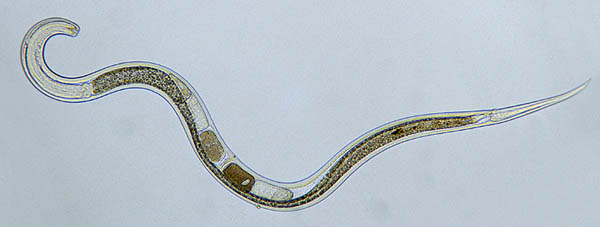
\includegraphics[width=0.28\textwidth]{../data/taxa_images/Nematoda_image.jpg}
    \caption{Nematoda}
    \label{fig:nematoda}
\end{wrapfigure}
\noindent\textbf{Nematoda} (F = 5.71**) decreased progressively from Cluster 0 (3.478) to Cluster 1 (2.468) to Cluster 2 (1.283). Roundworms show distinct habitat preferences based on sediment characteristics and organic matter content. They occupy multiple trophic levels as bacterivores, fungivores, and predators, making them important components of the meiofaunal community in aquatic sediments. \lipsum[6][1-4]

\begin{wrapfigure}{r}{0.3\textwidth}
    \centering
    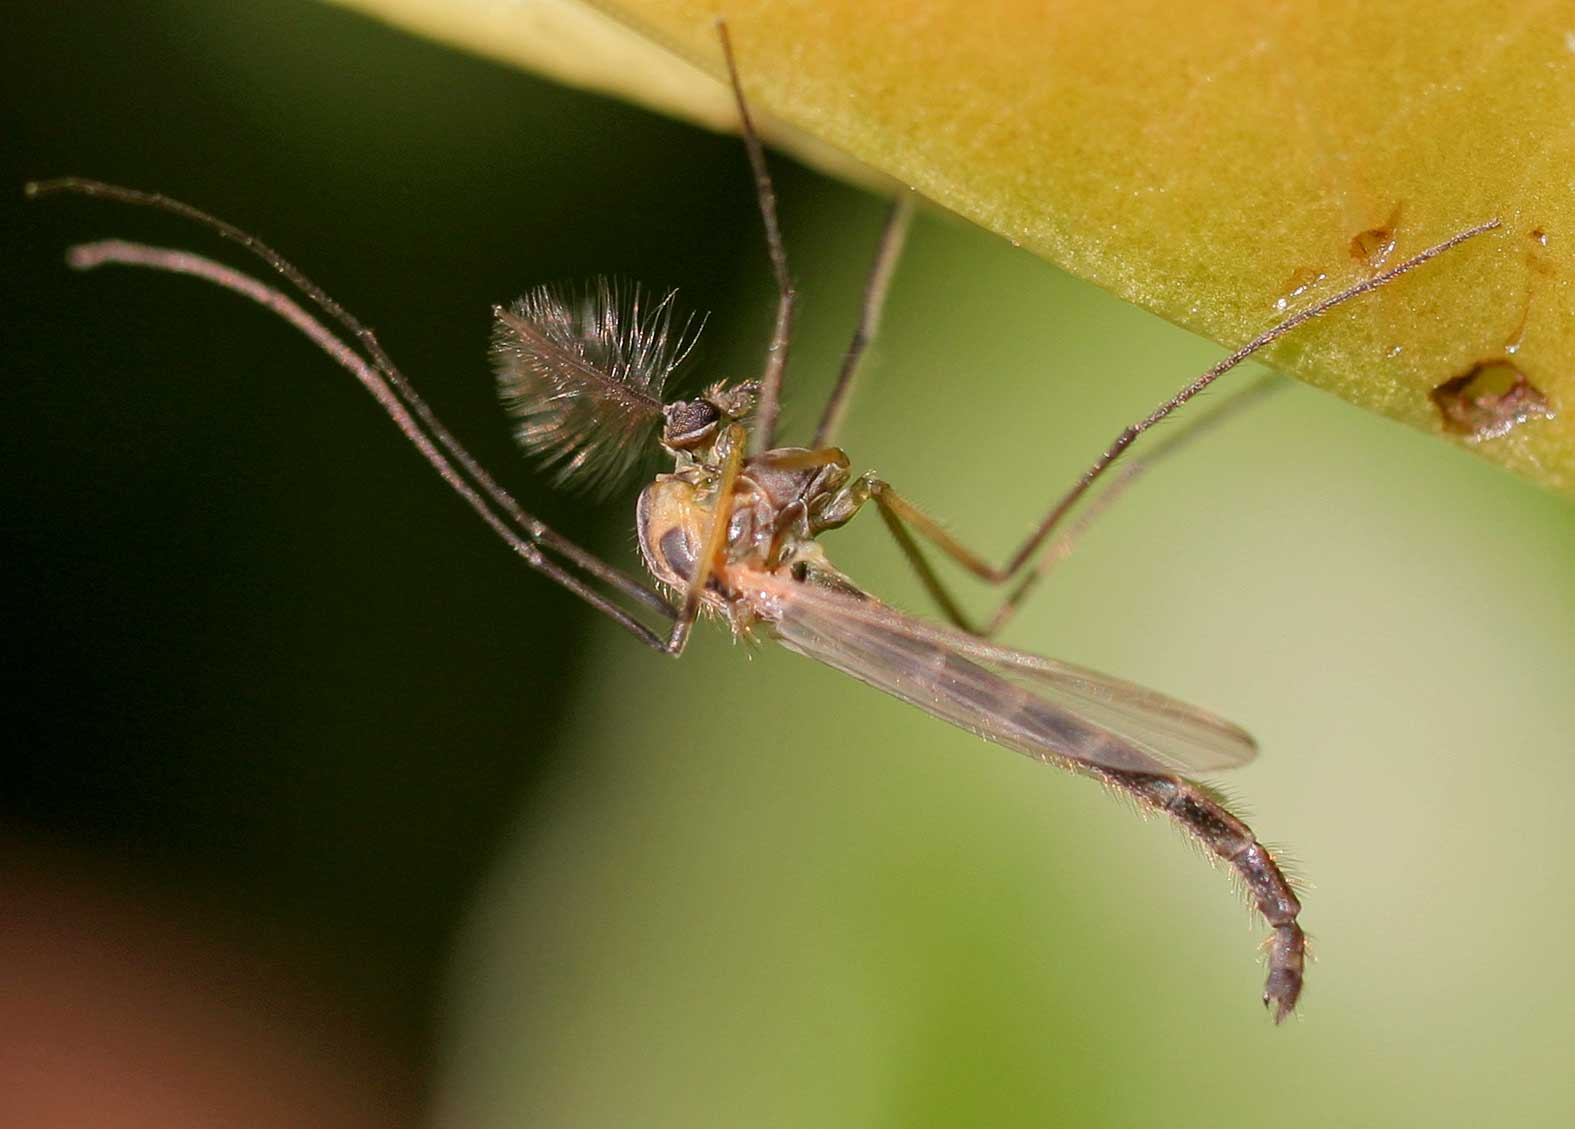
\includegraphics[width=0.28\textwidth]{../data/taxa_images/Chironomidae_image.jpg}
    \caption{Chironomidae}
    \label{fig:chironomidae}
\end{wrapfigure}
\noindent\textbf{Chironomidae} (F = 4.90*) showed lowest abundance in Cluster 0 (3.365) compared to Clusters 1 (4.689) and 2 (4.471). Non-biting midge larvae occupy a wide range of habitats with varying pollution tolerances. Different chironomid subfamilies and genera show distinct environmental preferences, making them valuable bioindicators when identified to lower taxonomic levels. \lipsum[7][1-4]


